% !TEX root = ../main.tex
\chapter{Commodity Models}\label{ch:commodities}
\begin{paracol}{2}

\begin{sources}
\begin{tabularx}{\linewidth}{@{}l l L@{}}
\toprule
\textbf{Lecture} & \textbf{Speaker} & \textbf{Content}\\
\midrule
2013 L13 & A.~Eydeland (Morgan Stanley) & What quants do in commodity markets: contango and the Trafigura trade; storage as a portfolio of calendar-spread options and the storage-optimisation problem; the power plant as a strip of spark-spread options; fat tails and spikes of power prices; why spot models fail; the ``stack'' (supply and demand) model of power prices.\\
\bottomrule
\end{tabularx}

\smallskip
\textbf{Files.} Slides \file{MIT18_S096F13_lecnote13.pdf} (47 pages: 44 of content, then references and disclaimers). \textbf{Problem sets.} None; all exercises at the end
are \emph{not from the course}. \textbf{Year.} Part~II of these notes collects the 2013-only topics; there is no 2024 counterpart. The guest is Alexander Eydeland (the
slides cite his book with K.~Wolyniec, \emph{Energy and Power Risk Management}, Wiley 2002, and a chapter with H.~Geman).
\textbf{Not in the slides.} The whole discussion of the trade, of the bid for storage and of the correlation structure comes from the video; the slides give the formulas
and the pictures. The sections marked \emph{(not discussed in class)} are additions of these notes, needed to make the lecture's claims precise
(Sections~\ref{ch21:sec-carry}, \ref{ch21:sec-schwartz} and part of \ref{ch21:sec-stats}, \ref{ch21:sec-stack}).
\end{sources}

\section*{Motivation}
Every other lecture of the course prices financial claims whose underlying can be bought, held and sold at negligible cost. A commodity is different: oil sits in tanks, gas in
salt caverns, electricity nowhere (it cannot be stored at scale). The quantities that matter are therefore physical: how much can be stored and how fast it can be injected, how
efficiently a plant turns fuel into power, what the supply curve of generators looks like. Eydeland's message is that the mathematics of derivatives
(\cref{ch:bs}) applies, but the \emph{objects} to be valued are physical assets, and each asset turns out to be a portfolio of options on a \emph{spread}:
\begin{center}
\small\begin{tabular}{@{}l l l@{}}
\toprule
asset & underlying spread & option\\
\midrule
oil or gas storage & calendar spread $F(T_2)-F(T_1)$ & \Cref{ch21:sec-spread}\\
gas-fired power plant & power $-$ heat rate $\times$ gas (spark spread) & \Cref{ch21:sec-plant}\\
refinery & products $-$ crude (crack spread) & \Cref{ch21:sec-assets}, \cref{ch09:sec-crack}\\
\bottomrule
\end{tabular}
\end{center}
The plan of the chapter is that of the lecture: a trade in a contango market (\cref{ch21:sec-carry}); the value of storage, the Margrabe spread-option formula and how
to hedge it (\cref{ch21:sec-spread,ch21:sec-storage}); the merchant power plant (\cref{ch21:sec-plant}); why power prices resist the standard spot models
(\cref{ch21:sec-stats,ch21:sec-schwartz}) and the alternative that models supply and demand (\cref{ch21:sec-stack}). The chapter uses the forward and futures
language of \cref{ch:rates} (futures are margined, forwards are not) and of \cref{ch15:prop-fwd}, the Black--Scholes machinery of \cref{ch:bs}, and the
Ornstein--Uhlenbeck process of \cref{ch:sde}; the crack-spread example of \cref{ch09:sec-crack} is the same economic object as the refinery above.

% ==================================================================
\section{Contango, backwardation and cash-and-carry}\label{ch21:sec-carry}

The lecture opens with a news item of March 2009: the trading house Trafigura expects its best results ever \emph{because} oil prices are low and the market is in contango
\ts{13}{13}{1:06}. A year earlier oil had reached \$159 per barrel and traders had been blamed for it; in 2009 it fell to about \$30 and the same traders made record profits
\ts{13}{13}{2:07}. The apparent paradox is resolved by looking at the futures curve.

\subsection{The futures curve}
A \emph{futures contract} lets one buy today, at a price fixed today, a barrel to be delivered at a future date; the prices $F(t,T)$ for all maturities $T$ form the
\emph{futures} (or \emph{forward}) \emph{curve} \ts{13}{13}{3:09}. In commodity markets there is no ``spot price'' as such: what television calls the spot price is the price of the
nearest futures contract \ts{13}{13}{4:10}.

\begin{definition}[Contango and backwardation]\label{ch21:def-contango}
The curve $T\mapsto F(t,T)$ is in \emph{contango} if it is increasing and in \emph{backwardation} if it is decreasing \ts{13}{13}{4:10}. (Loosely, one says that the market is
in contango or backwardation when the curve is so at the front, i.e.\ when $F(t,T)\gtrless S_t$.)
\end{definition}

On 15 January 2009 the WTI curve was in steep contango: about \$35 for the nearest contract (February 2009), \$55 for August, \$58 for December and \$60 for February 2010
(\cref{ch21:fig-wti}; the intermediate points are read off the slide and are approximate).

\begin{figure}[ht]
\centering
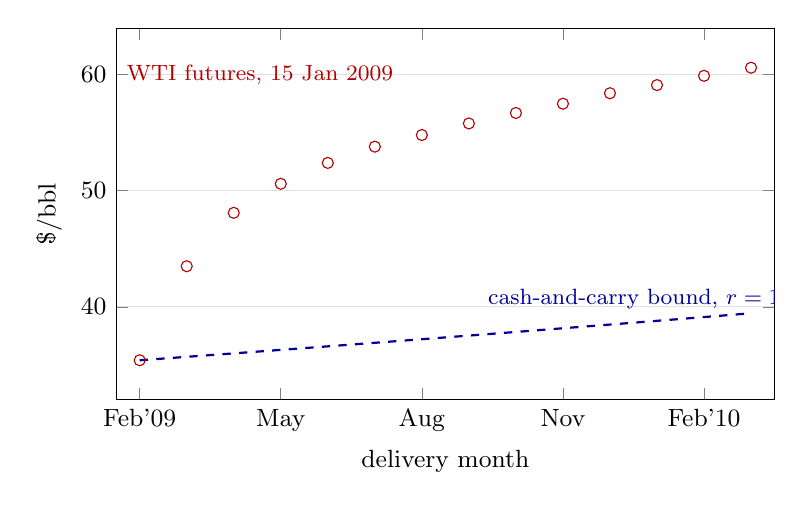
\begin{tikzpicture}
\begin{axis}[width=0.82\linewidth,height=6.3cm,xlabel={delivery month},ylabel={\$/bbl},xmin=-0.5,xmax=13.5,ymin=32,ymax=64,
  xtick={0,3,6,9,12},xticklabels={Feb'09,May,Aug,Nov,Feb'10},ymajorgrids,grid style={black!12},tick label style={font=\small},label style={font=\small}]
\addplot[only marks,mark=o,red!70!black,mark size=2pt] coordinates {(0,35.4) (1,43.5) (2,48.1) (3,50.6) (4,52.4) (5,53.8) (6,54.8) (7,55.8) (8,56.7) (9,57.5) (10,58.4) (11,59.1) (12,59.9) (13,60.6)};
\addplot[thick,dashed,blue!60!black,domain=0:13,samples=27] {35.4*exp(0.10*x/12)};
\node[font=\footnotesize,blue!60!black,anchor=west] at (axis cs:7.2,40.7) {cash-and-carry bound, $r=10\%$};
\node[font=\footnotesize,red!70!black,anchor=east] at (axis cs:5.6,60.0) {WTI futures, 15 Jan 2009};
\end{axis}
\end{tikzpicture}
\caption{The WTI futures curve of 15 January 2009 (points read off slide~4 of the lecture) against the upper bound $S\,e^{rT}$ that a holder of free storage would impose with $r=10\%$
(\cref{ch21:prop-carry}). The gap between the two is what the market charges for storage.}\label{ch21:fig-wti}
\end{figure}

\subsection{The Trafigura trade}
Suppose one owns storage. Then on 15 January 2009 one can, at no risk \ts{13}{13}{5:11}\ts{13}{13}{6:16}:
\begin{enumerate}[1.]
  \item borrow \$35 and buy one barrel (the nearby price);
  \item store it for a year;
  \item sell one February-2010 futures contract, fixing the sale price at \$60.
\end{enumerate}
The lock-in is $60-35=\$25$ minus the interest on the loan: \$3.5 at 10\% simple interest, so a profit of \$21.5 per barrel (the lecturer says ``about 21''); with continuous compounding the
interest is $35(e^{0.10}-1)=3.68$ and the profit \$21.3. With 50--60 million barrels of storage the total is enormous and risk-free \ts{13}{13}{6:16}. The trade needs
low prices \emph{because} the interest is proportional to the price paid: at \$125--160 a barrel the same contango would leave about half the profit \ts{13}{13}{7:21}. What it needs
is \emph{storage}: the strategy is ``long the February 2009 contract, short the February 2010 contract'', i.e.\ a long \emph{calendar spread}, plus a tank to receive the
barrel \ts{13}{13}{7:21}.

\begin{proposition}[Cash-and-carry bounds]\label{ch21:prop-carry}
Let the interest rate $r$ and the storage cost rate $u$ (proportional to the price, per unit time) be constant, and let $S$ be the price of the physical commodity, which is
storable. In the absence of arbitrage for an agent that can store,
\[
  F(0,T)\ \le\ S_0\,e^{(r+u)T}.
\]
\end{proposition}
\begin{proof}
If $F(0,T)>S_0e^{(r+u)T}$, borrow $S_0$, buy the commodity, pay the storage cost, and sell the future. At $T$ deliver against $F(0,T)$ and repay the loan with its interest
and the accumulated storage cost $S_0e^{(r+u)T}$: the net cash flow $F(0,T)-S_0e^{(r+u)T}>0$ is certain and costs nothing. This is the argument of \cref{ch15:prop-fwd} with a storage cost.
\end{proof}
The opposite inequality $F\ge S_0e^{(r+u)T}$ does \emph{not} follow, because it would require selling the commodity today and buying it back later: only somebody who holds inventory can do that,
and holding inventory may itself be valuable (a refinery that runs out of crude stops). The shortfall is captured by the \emph{convenience yield} $y$ defined by
\begin{equation}\label{ch21:eq-convenience}
  F(0,T)=S_0\,e^{(r+u-y)T},\qquad y=r+u-\frac1T\ln\frac{F(0,T)}{S_0}\ \ge 0\ \text{ for a storable commodity.}
\end{equation}
(Not discussed in class.) Backwardation corresponds to a large convenience yield, $y>r+u$: inventory is scarce and valuable, spot is expensive against later delivery.

\begin{example}[The 2009 contango]\label{ch21:ex-implied}
With $S_0=35$, $F=60$ and $T=1$ year the implied cost of carry is $\ln(60/35)=54\%$ per year: at $r=10\%$ the bound of \cref{ch21:prop-carry} would require $u\ge44\%$ per year to remove the
arbitrage, i.e.\ $y=r+u-0.539<0$ for any reasonable $u$. The resolution is that the arbitrage is available only to those who own \emph{empty storage}; storage was scarce
(the market was oversupplied) and its shadow price was the difference $60-35e^{0.10}=21.3$ per barrel per year. Contango of this size is the market's bid for tanks.
\end{example}

\begin{finance}[Physical assets and \emph{who} can arbitrage]
The arbitrage of \cref{ch21:prop-carry} is not open to a financial investor: without storage one cannot take the physical leg. Contango therefore pays the owners of scarce
infrastructure (tanks, supertankers used as floating storage, salt caverns for gas) and the shape of the curve is best read as the price of the option to store. The remainder
of the lecture asks the inverse question: given the curve, \emph{what is a tank worth?}
\end{finance}

\begin{intuition}[Physicist's reading]
Think of the curve as a potential energy landscape along the time axis. A steep upward slope in $T$ is a gradient that an owner of storage can ``roll down'' at fixed cost: buy at the
bottom, sell at the top. Backwardation is the reversed slope: the tank owner is paid to empty the tank now and refill it later. The convenience yield is the price of the dissipation that keeps
the slope from exceeding $r+u$ when storage is plentiful.
\end{intuition}

% ==================================================================
\section{The value of storage: a calendar-spread option}\label{ch21:sec-spread}

\subsection{The bid for a tank}
The lecturer inverts the question \ts{13}{13}{7:21}\ts{13}{13}{8:21}. Your boss hands you a credit card and asks you to obtain storage from August to December in an auction, with the same
curve: $F_{\mathrm{Aug}}=55$, $F_{\mathrm{Dec}}=58$. Bid too little and you lose; bid too much and you suffer the winner's curse. The maximal bid is the amount that one can be \emph{sure to recover},
so a bidder needs, before bidding, a strategy that recovers the price paid \ts{13}{13}{9:23}.

\paragraph{The trader's answer.} Buy the August contract and sell the December contract on 1 January; on 1 August take delivery of the barrel and store it; in December deliver against the
December contract. This locks $58-55=3$ dollars per barrel: one can pay up to \$3 (say \$2.99, to keep a penny of profit) \ts{13}{13}{10:25}\ts{13}{13}{11:31}\ts{13}{13}{12:35}. Interest is ignored
``for simplicity'' (slide~9 adds: it should not be) \ts{13}{13}{11:31}. With interest at rate $r$ the locked amount, in December dollars, is $F_{\mathrm{Dec}}-F_{\mathrm{Aug}}e^{r(T_{\mathrm{Dec}}-T_{\mathrm{Aug}})}$, since the \$55 paid in August must be financed until the sale: at $r=10\%$ and four months the financing costs about
$55(e^{0.10/3}-1)\approx1.9$, more than half of the locked \$3, which is why the lecturer says that one must not really forget it.

\paragraph{The quant's answer.} On 1 January sell to somebody an \emph{August--December calendar spread option}, exercised on 31 July, with payoff
\begin{equation}\label{ch21:eq-payoff}
  \bigl[F_{\mathrm{Dec}}(T)-F_{\mathrm{Aug}}(T)\bigr]^+,\qquad T=\text{31 July},
\end{equation}
the futures prices being those quoted on the exercise date \ts{13}{13}{12:35}\ts{13}{13}{13:38}. There is no strike: the ``strike'' is the other futures price, so the option is a function of two random
variables and is more difficult than an option on a single stock \ts{13}{13}{14:39}. Using the formula of \cref{ch21:thm-margrabe} below, the lecture quotes $V=4.4677$ dollars per barrel
\ts{13}{13}{15:39}. So one can bid, for instance, \$4.20 \ts{13}{13}{15:39}: the bid beats the trader's ceiling of \$3, and the margin ($4.4677-4.20=0.27$) is much larger than a penny.

Why is the value larger than the \$3 of the trader? Because $3=F_{\mathrm{Dec}}-F_{\mathrm{Aug}}$ is the \emph{intrinsic value} of the option, its value at zero volatility, and an option is worth more than its
intrinsic value when the volatility is positive; energy volatilities are far larger than in rates, currencies or equity indices \ts{13}{13}{16:44}.

\paragraph{Where is the risk?} Selling the option exposes one to an unbounded payment. Suppose on 31 July $F_{\mathrm{Aug}}=55$ and $F_{\mathrm{Dec}}=80$ (slide~11 uses $65$ and $80$): the seller owes \$25 (slide: \$15)
\ts{13}{13}{17:47}. But he owns the tank: he buys August and sells December \emph{at the same moment} using futures, and later moves the physical barrel, collecting exactly $F_{\mathrm{Dec}}-F_{\mathrm{Aug}}$
\ts{13}{13}{18:48}\ts{13}{13}{19:54}. If instead December falls below August the option pays nothing and the tank is left unused \ts{13}{13}{20:55}. So the tank \emph{is} the option: a full hedge, whatever happens.

\subsection{The spread-option formula}
The value quoted on slide~10 is the formula for an option to exchange one lognormal asset for another (Margrabe, 1978), applied to two futures prices. The natural setting is that of \cref{ch15:sec-rn}:
futures are costless to enter and margined daily, so under the risk-neutral measure $\Q$ a futures price is a martingale (the futures analogue of the statement that the discounted stock is a martingale).

\begin{theorem}[Zero-strike spread option; Margrabe]\label{ch21:thm-margrabe}
Let $F_1,F_2$ be $\Q$-martingales with $\dd F_i=\sigma_iF_i\dd W_i$, $\dd W_1\dd W_2=\rho\dd t$, constant $\sigma_i>0$ and $|\rho|<1$, and let the discount factor to the expiry $T$ be $e^{-rT}$. Then
\begin{equation}\label{ch21:eq-margrabe}
  V=e^{-rT}\,\E_\Q\bigl[(F_2(T)-F_1(T))^+\bigr]=e^{-rT}\bigl[F_2(0)\,\Phi(d_1)-F_1(0)\,\Phi(d_2)\bigr],
\end{equation}
\[
  d_1=\frac{\ln\bigl(F_2(0)/F_1(0)\bigr)+\tfrac12\sigma^2T}{\sigma\sqrt T},\quad d_2=d_1-\sigma\sqrt T,\quad \sigma^2=\sigma_1^2+\sigma_2^2-2\rho\sigma_1\sigma_2,
\]
and $\Phi$ is the standard normal distribution function. (Slide 10, with ``DiscFactor'' $=e^{-rT}$ and $N=\Phi$.)
\end{theorem}
\begin{proof}
Write $(F_2-F_1)^+=F_1(T)\,(X_T-1)^+$ with $X=F_2/F_1$. Define a new measure $\Q^1$ on $\mathcal F_T$ by $\dd\Q^1/\dd\Q=F_1(T)/F_1(0)$, a positive random variable of mean one because $F_1$ is a
$\Q$-martingale. Then
\[
  \E_\Q\bigl[F_1(T)(X_T-1)^+\bigr]=F_1(0)\,\E_{\Q^1}\bigl[(X_T-1)^+\bigr].
\]
Under $\Q^1$ the ratio $X$ is a martingale: for $A\in\mathcal F_t$,
\[
\begin{gathered}
\E_{\Q^1}[X_T\ind_A]=\E_\Q\bigl[F_1(T)F_1(0)^{-1}F_2(T)F_1(T)^{-1}\ind_A\bigr]=\E_\Q[F_2(T)\ind_A]/F_1(0)\\
=\E_\Q[F_2(t)\ind_A]/F_1(0)=\E_{\Q^1}[X_t\ind_A].
\end{gathered}
\]
By Ito's formula $\dd X/X=\sigma_2\dd W_2-\sigma_1\dd W_1+(\text{drift})\dd t$, with quadratic variation $(\sigma_1^2+\sigma_2^2-2\rho\sigma_1\sigma_2)\dd t=\sigma^2\dd t$; the volatility of a process does not change when we change to an equivalent measure
(as recalled after \cref{ch15:eq-rnval}), and the drift is then forced by the martingale property. So $X$ is a driftless lognormal, $X_T=X_0e^{-\sigma^2T/2+\sigma\sqrt T Z}$ under $\Q^1$, and the Black formula with unit strike and zero rate (\cref{ch15:thm-bs})
gives $\E_{\Q^1}[(X_T-1)^+]=X_0\Phi(d_1)-\Phi(d_2)$. Multiplying by $F_1(0)$ gives~\eqref{ch21:eq-margrabe}.
\end{proof}

The proof used only that the \emph{ratio} is lognormal; the numeraire is the asset $F_1$ (this change-of-numeraire trick is the standard proof of Margrabe's formula). Three properties are immediate.

\begin{proposition}[Properties]\label{ch21:prop-props}
\leavevmode
\begin{enumerate}[(i)]
  \item $V\ge e^{-rT}(F_2(0)-F_1(0))^+$, with equality in the limit $\sigma\to0$: the option is worth at least its intrinsic value (Jensen, since $F_2-F_1$ is a martingale and $x\mapsto x^+$ is convex).
  \item $V$ is homogeneous of degree one in $(F_1,F_2)$ and increasing in $\sigma$, and depends on $(\sigma_1,\sigma_2,\rho)$ only through the \emph{spread volatility} $\sigma$; in particular a \emph{higher} correlation $\rho$ \emph{lowers} the value.
  \item The derivatives are $\partial V/\partial F_2=e^{-rT}\Phi(d_1)$ and $\partial V/\partial F_1=-e^{-rT}\Phi(d_2)$.
\end{enumerate}
\end{proposition}
\begin{proof}
(i) is Jensen.

(ii) Degree one is visible in~\eqref{ch21:eq-margrabe}; the vega is $e^{-rT}F_2\varphi(d_1)\sqrt T>0$ ($\varphi$ the normal density; the same computation as the vega of \cref{ch:bs}).

(iii) Differentiating,
$\partial_{F_2}V=e^{-rT}[\Phi(d_1)+(F_2\varphi(d_1)-F_1\varphi(d_2))\,\partial_{F_2}d_1]$ (using $d_2=d_1-\sigma\sqrt T$), and the bracket vanishes because
$\varphi(d_2)/\varphi(d_1)=e^{d_1\sigma\sqrt T-\sigma^2T/2}=F_2/F_1$. The other derivative follows by Euler's identity $V=F_1\partial_1V+F_2\partial_2V$ for degree-one functions.
\end{proof}

\paragraph{The numbers of slide 10.} The slide gives neither the volatilities, nor the correlation, nor the time to expiry. Taking the exercise date 31 July, $T=211/365=0.578$ years from 1 January, and
zero interest, one finds that $\sigma_1=\sigma_2=50\%$ and $\rho=0.95$ reproduce the printed value: $\sigma=0.5\sqrt{2(1-0.95)}=0.1581$ and
\[
  V=58\,\Phi(0.5019)-55\,\Phi(0.3817)=58\cdot0.6921-55\cdot0.6486=4.4677
\]
to four decimals (verified numerically; solving directly for $\sigma$ gives $0.15811$). This is our reconstruction, not something said in the lecture. The value splits as $3.00$ of intrinsic and $1.47$ of time value. The dependence on the correlation
is dramatic (\cref{ch21:tab-rho}): $\rho=1$ gives exactly the intrinsic value, and a fall of $\rho$ from $0.99$ to $0.95$ raises the value by $1.2$ dollars.

\begin{table}[ht]
\centering
\begin{tabular}{@{}l r r r r r r@{}}
\toprule
$\rho$ & $1$ & $0.99$ & $0.98$ & $0.95$ & $0.90$ & $0.80$\\
\midrule
$\sigma$ (spread vol.) & $0$ & $0.0707$ & $0.1000$ & $0.1581$ & $0.2236$ & $0.3162$\\
$V$ (\$/bbl) & $3.000$ & $3.259$ & $3.615$ & $4.468$ & $5.512$ & $7.037$\\
\bottomrule
\end{tabular}
\caption{Aug--Dec spread option, $F_{\mathrm{Aug}}=55$, $F_{\mathrm{Dec}}=58$, $T=211/365$, $r=0$, $\sigma_1=\sigma_2=50\%$. Computed for these notes.}\label{ch21:tab-rho}
\end{table}

\begin{figure}[ht]
\centering
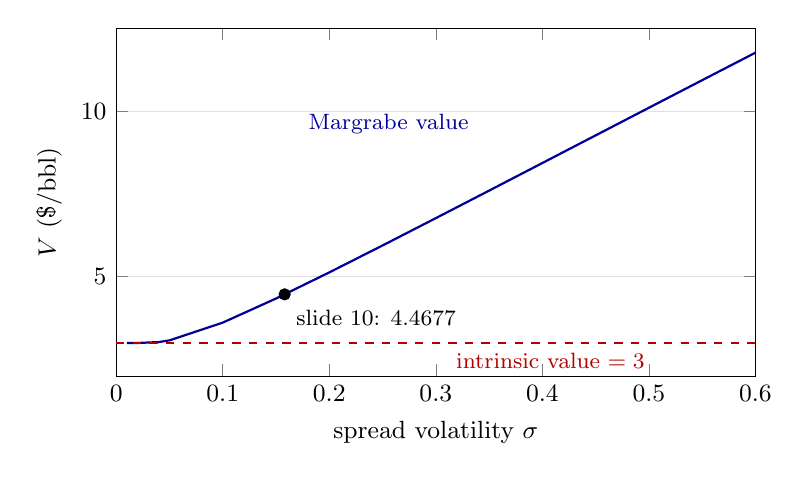
\begin{tikzpicture}
\begin{axis}[width=0.8\linewidth,height=6cm,xlabel={spread volatility $\sigma$},ylabel={$V$ (\$/bbl)},xmin=0,xmax=0.6,ymin=2,ymax=12.5,ymajorgrids,grid style={black!12},tick label style={font=\small},label style={font=\small}]
\addplot[thick,blue!60!black] coordinates {(0.01,3.0000) (0.02,3.0001) (0.04,3.0280) (0.05,3.0792) (0.1,3.6148) (0.15,4.3425) (0.2,5.1305) (0.25,5.9434) (0.3,6.7680) (0.35,7.5985) (0.4,8.4318) (0.45,9.2659) (0.5,10.0995) (0.55,10.9318) (0.6,11.7620)};
\addplot[dashed,red!70!black,domain=0:0.6] {3};
\node[font=\footnotesize,red!70!black,anchor=north west] at (axis cs:0.31,3.0) {intrinsic value $=3$};
\node[font=\footnotesize,blue!60!black,anchor=east] at (axis cs:0.34,9.6) {Margrabe value};
\addplot[only marks,mark=*,mark size=2pt,black] coordinates {(0.15811,4.4677)};
\node[font=\footnotesize,anchor=north west] at (axis cs:0.16,4.3) {slide 10: $4.4677$};
\end{axis}
\end{tikzpicture}
\caption{Value of the August--December spread option as a function of the spread volatility, for $F=(55,58)$, $T=211/365$, no interest. The dot is the number printed on slide~10.}\label{ch21:fig-vol}
\end{figure}

\begin{remark}[Why correlation between contract months is the model's hard part]
The value of a calendar-spread option depends on the joint law of two points of the forward curve, in particular on their correlation (\cref{ch21:tab-rho}). A model that generates all forward prices from one random factor gives
$\rho=1$ and hence an option worth its intrinsic value: it cannot price the storage. This is the content of the slide-31 objection ``cannot model the correlation structure between forward contracts'' and is made
precise in \cref{ch21:sec-schwartz}.
\end{remark}

\begin{coursenote}[Errata and inconsistencies in this part]
\begin{itemize}
  \item Slide~11 repeats the example with $F_{\mathrm{Aug}}=65$, $F_{\mathrm{Dec}}=80$ (owe \$15) while the lecturer speaks of 55 and 80 (owe \$25); both are consistent examples.
  \item Slide~11 says the bid can be raised to \$4.46, the truncation of $4.4677$ (the lecturer says 447 cents and bids
      420).
  \item Slide~5 gives the profit of the Trafigura trade as \$21.5 with 10\% \emph{simple} interest, the speaker says ``21''.
  \item Slide~9 says ``interest rates are ignored for simplicity (should not be)'': formula~\eqref{ch21:eq-margrabe} holds with the discount factor, but the trader's static ceiling of \$3
      needs the financing correction above.
\end{itemize}
\end{coursenote}

% ==================================================================
\section{Hedging the tank, and the real storage problem}\label{ch21:sec-storage}

\subsection{There is no market: replicate}\label{ch21:sec-hedge}
The lecture makes a confession \ts{13}{13}{37:39}: there is no market for spread options, nobody will buy the option that the quant ``sold'' for 4.4677. What survives is the
\emph{method} behind Black--Scholes: the value is also the cost of a dynamic strategy that reproduces the payoff \ts{13}{13}{38:43}\ts{13}{13}{39:49}. The quant therefore does not sell anything; he owns the tank,
whose payoff is that of the option, and delta-hedges it, and he tells the trader what to do every day, and the tank operator when to inject and withdraw \ts{13}{13}{40:49}.

To make this precise (the lecture does not write it down) let $V(F_1,F_2)$ be the value~\eqref{ch21:eq-margrabe}. \emph{Owning} the option (the tank) and hedging means holding $-\Phi(d_1)$ Dec futures and $+\Phi(d_2)$
Aug futures, by \cref{ch21:prop-props}(iii) rebalanced continuously. Futures cost nothing to hold, so the hedge earns $-\Phi(d_1)\dd F_2+\Phi(d_2)\dd F_1$ and the terminal value of the whole position is
\[
\begin{gathered}
  \bigl(F_2(T)-F_1(T)\bigr)^+-\int_0^T\Phi(d_1)\dd F_2+\int_0^T\Phi(d_2)\dd F_1=V(F_1(0),F_2(0))\\
  \text{(continuous rebalancing, } r=0),
\end{gathered}
\]
the standard Black--Scholes replication statement (\cref{ch:bs}): Ito's formula applied to $V(F_1,F_2)$, which solves the two-dimensional Black equation with terminal
condition~\eqref{ch21:eq-payoff}, gives $\dd V=\partial_{F_1}V\dd F_1+\partial_{F_2}V\dd F_2$ (time-derivative and second-order terms cancel).
The hedger who wins the tank at price $P<V$ therefore locks in $V-P$. When the option ends in the money both deltas tend to one: the hedge is ``long August, short December'', exactly the
trader's static position of \cref{ch21:sec-spread}, which the tank then converts into physical barrels. In this sense the trader's strategy is the limit $\sigma\to0$ of the quant's.

\begin{table}[ht]
\centering
\begin{tabular}{@{}l r r r r r@{}}
\toprule
hedging dates $n$ & $1$ & $4$ & $16$ & $64$ & $211$\\
\midrule
mean of final P\&L & $4.462$ & $4.466$ & $4.472$ & $4.469$ & $4.468$\\
standard deviation & $2.033$ & $1.078$ & $0.567$ & $0.290$ & $0.159$\\
\bottomrule
\end{tabular}
\caption{Discrete delta-hedging of the option of \cref{ch21:tab-rho} ($\sigma_1=\sigma_2=50\%$, $\rho=0.95$; $V=4.4677$): terminal payoff plus hedge P\&L. Computed for these notes: $2\cdot10^4$ paths, $n$ equally spaced dates between 1 January and 31 July, no interest.}\label{ch21:tab-hedge}
\end{table}
The simulation (\cref{ch21:tab-hedge}) shows the two things one expects: the average of the final position is the premium $V$ whatever $n$, and the residual risk falls like $n^{-1/2}$, from $2.0$ dollars per barrel with a single rebalancing to $0.16$ with daily hedging.

\begin{remark}
The storage owner is \emph{long} the option, while the lecture speaks of ``selling'' it and covering the short position with the tank. The two views are the same portfolio seen from the two sides: sold option plus tank is riskless with value $V-P$; the hedge of the previous
paragraph reaches the same result without a counterparty. A subtlety: the option is settled on 31 July on the \emph{futures} prices, while the barrels move later, so between the two dates the operator is committed by the futures he has entered, which is why the recipe ``buy August, sell December at the same time'' works.
\end{remark}

\subsection{A portfolio of options under physical constraints}\label{ch21:sec-portfolio}
A real tank is available for two years, not for four months, and one may sell many spread options against it: injection in any month $T_i$ and withdrawal in any later month $T_j$, and also the opposite (withdraw first, refill later), which pays when the curve is
in backwardation \ts{13}{13}{21:58}\ts{13}{13}{27:11}. The first problem is to choose \emph{which portfolio of options} is the most valuable one that the tank can support, and this is an optimisation \ts{13}{13}{23:00}. The constraints are
technical, contractual and legal: injection and withdrawal rates, tank capacity, and above all the requirement that \emph{under no circumstances} the tank is asked to do something impossible \ts{13}{13}{24:02}\ts{13}{13}{25:05}. Slides 13--17 write the problem
as follows. With dates $T_1<\dots<T_N$ and today's futures prices $F_i$ (slide~13):
\begin{itemize}
  \item $S_{i,j}$ ($i<j$) is the value of the option to inject at $T_i$ and withdraw at $T_j$, with payoff $\max\{F_j-F_i-\mathrm{Cost},0\}$ at exercise; $U_{i,j}$ the value of the option to withdraw at $T_i$ and inject at the later
        $T_j$, with payoff $\max\{F_i-F_j-\mathrm{Cost},0\}$ (slide~14) \ts{13}{13}{27:11}\ts{13}{13}{28:16}. The volumes sold against the tank are $x_{i,j}\ge0$ and $\nu_{i,j}\ge0$;
  \item $y_i\ge0$ and $z_j\ge0$ are the volumes committed today by \emph{futures} for injection at $T_i$ and withdrawal at $T_j$ (the trader's static strategy);
  \item the objective is the cash collected now:
\begin{equation}\label{ch21:eq-storage-obj}
\begin{gathered}
  V=\max_{x,\nu,y,z}\Bigl\{\sum_{i<j}x_{i,j}S_{i,j}+\sum_{i<j}\nu_{i,j}U_{i,j}-\sum_iy_iF_i+\sum_jz_jF_j\Bigr\}\\
  \ts{13}{13}{25:05}\ts{13}{13}{26:11}
\end{gathered}
\end{equation}
        (the first two sums are premia received, the last two are the cost of the futures bought to inject and the revenue of the futures sold to withdraw);
  \item Boolean variables record the exercise: $\Omega^S_{i,j}=1$ if $S_{i,j}$ expires in the money (then the tank \emph{must} act), $0$ otherwise, and the same for $\Omega^U_{i,j}$ \ts{13}{13}{28:16}\ts{13}{13}{29:18}.
\end{itemize}
Define the net injection at date $T_i$ (positive means into the tank)
\begin{equation}\label{ch21:eq-qi}
  q_i=\sum_{j>i}x_{i,j}\Omega^S_{i,j}-\sum_{\ell<i}x_{\ell,i}\Omega^S_{\ell,i}+\sum_{\ell<i}\nu_{\ell,i}\Omega^U_{\ell,i}-\sum_{j>i}\nu_{i,j}\Omega^U_{i,j}+y_i-z_i .
\end{equation}
An exercised option of type~$S$ injects $x_{i,j}$ at $T_i$ and withdraws it at $T_j$, so the two terms cancel if both legs fall on the same date (a withdrawal already required cancels an injection required now, \ts{13}{13}{30:19}); for type~$U$ the signs
are reversed. The constraints of slides 16--17 are then
\begin{align}
  &-W_i\ \le\ q_i\ \le\ I_i, && i=1,\dots,N &&\text{(withdrawal and injection rates)}\label{ch21:eq-rates}\\
  &C^{\min}_i\ \le\ C_0+\sum_{k\le i}q_k\ \le\ C^{\max}_i, && i=1,\dots,N &&\text{(capacity)}\label{ch21:eq-cap}
\end{align}
where $C_0$ is the initial inventory. On slide~17 the capacity constraint is written $C_0+\sum_{k\le i}\{\sum_{j>i}x_{k,j}\Omega^S_{k,j}-\sum_{j>i}\nu_{k,j}\Omega^U_{k,j}+y_k-z_k\}$: this is the same thing, because in
$\sum_{k\le i}q_k$ every pair $(k,j)$ with $k<j\le i$ contributes $+x_{k,j}$ at $T_k$ and $-x_{k,j}$ at $T_j$ and cancels, so only the pairs still open at $T_i$ (those with $j>i$) survive.

\begin{remark}[Why the problem is ugly]
The variables $\Omega$ depend on prices at the exercise dates: they are random. The constraints must hold in every price scenario, so \eqref{ch21:eq-rates}--\eqref{ch21:eq-cap} are in effect a \emph{robust} problem, one system for each of the $2^{n_{\mathrm{opt}}}$ exercise patterns.
The unknowns are $x,y,z,\nu$ and, unfortunately, the Boolean $\Omega$, and the constraints are non-linear in them \ts{13}{13}{31:20}. For two years of monthly dates there are $24\cdot23/2=276$ pairs of each type, plus an equally large
set of constraints \ts{13}{13}{32:24}. (The lecturer stumbles over the count; this is the count of pairs $i<j$. The reading of the constraints as a robust problem is ours.)
\end{remark}

\subsection{The linear core: intrinsic value}\label{ch21:sec-intrinsic}
If the option premia are removed and only the futures part is kept, the problem~\eqref{ch21:eq-storage-obj}--\eqref{ch21:eq-cap} with $x=\nu=0$ is a \emph{linear program}: it gives the \emph{intrinsic value} of the tank, what can be locked in with futures alone
(the trader's strategy, made rigorous). (Not discussed in class.) Take twelve monthly dates with the approximate curve of \cref{ch21:fig-wti} (February 2009 to January 2010), a tank with $C_0=0$, $C^{\max}=100$, injection rate $I=30$ and withdrawal rate $W=40$ per month,
no costs. Maximising $\sum_iF_i(z_i-y_i)$ subject to $0\le y_i\le I$, $0\le z_i\le W$ and $0\le\sum_{k\le i}(y_k-z_k)\le C^{\max}$ gives
\begin{center}
\footnotesize
\setlength{\tabcolsep}{3.2pt}
\begin{tabular}{@{}l r r r r r r r r r r r r@{}}
\toprule
month & Feb & Mar & Apr & May & Jun & Jul & Aug & Sep & Oct & Nov & Dec & Jan\\
$F_i$ & 35.4 & 43.5 & 48.1 & 50.6 & 52.4 & 53.8 & 54.8 & 55.8 & 56.7 & 57.5 & 58.4 & 59.1\\
inject $y_i$ & 30 & 30 & 30 & 10 & 0 & 0 & 0 & 0 & 0 & 0 & 0 & 0\\
withdraw $z_i$ & 0 & 0 & 0 & 0 & 0 & 0 & 0 & 0 & 0 & 20 & 40 & 40\\
\bottomrule
\end{tabular}
\end{center}
and an intrinsic value of $5850-4316=1534$ dollars (average purchase price $43.16$, average sale price $58.50$). Without the rate limits one would fill the tank in February for $3540$ and empty it in January for $5910$ (value $2370$): the injection limit alone
costs $836$, and the LP finds the cheapest way around it, filling in the cheap months first. (Computed for these notes with \texttt{scipy.optimize.linprog}.) The quant's value is this plus the value of the flexibility, the time value of the spread options.

\subsection{Methods, robustness and calibration}\label{ch21:sec-methods}
The lecture lists three ways to attack the full problem \ts{13}{13}{32:24}\ts{13}{13}{33:31}: approximate it by a linear or quadratic programme; Monte Carlo simulation of the prices; or \emph{stochastic control}, for which the reference is Carmona and Ludkovski (2010),
``Valuation of energy storage: an optimal switching approach'', \emph{Quantitative Finance} 10(4) (slide~18): the decision inject/withdraw/hold is a control chosen as a function of the current prices and inventory, and the value is the solution of a dynamic-programming equation. None of the methods is ``better'': the
inputs (volatilities, correlations) are known only to a rough accuracy, and an exact method fed with parameters that are 50\% off is still wrong \ts{13}{13}{33:31}\ts{13}{13}{34:35}.

\begin{finance}[Robust, calibration-free models]
Eydeland's desk, in his words, does not use the stochastic-control solution (``we do something different'') and deliberately chooses a method that is \emph{robust}: little changes in the parameters must not change the value much, and each ingredient must be
something that can be traded in the market and verified by outside controllers and regulators, ``in this day and age extremely important'' \ts{13}{13}{34:35}\ts{13}{13}{35:35}. He warns against over-parametrised models (stochastic volatility, regime switching, several jump processes),
which capture the richness of price behaviour at the cost of stability \ts{13}{13}{35:35}. \emph{Calibration}, the fitting of unobservable parameters by least squares to market data, is fragile: the objective is non-convex, the solution set can be very flat, one may stop early
\ts{13}{13}{36:35}\ts{13}{13}{37:39}. Compare the regularisation of ill-posed calibration problems in \cref{ch:regularized} and the least-squares theory of \cref{ch:regression}.
\end{finance}

% ==================================================================
\section{The merchant power plant and the spark spread}\label{ch21:sec-plant}

\subsection{A plant is a strip of daily options}
The same reasoning applies to any physical asset: tankers, refineries, pipelines, power lines \ts{13}{13}{41:53}; only the constraints change (a tanker needs the routes and port limits) \ts{13}{13}{42:59}. The second half of the lecture works out the power plant.

A \emph{merchant} plant decides itself, every morning, whether to run \ts{13}{13}{42:59}\ts{13}{13}{44:00}. The price of power for the day is known; to produce one megawatt-hour it burns fuel. The efficiency is measured by the \emph{heat rate} $h$:
the number of MMBtu of fuel per MWh (typically 7 for a modern gas plant, up to 20 for an inefficient one that runs rarely) \ts{13}{13}{45:05}\ts{13}{13}{46:09}. With the fuel price $G$ (dollars per MMBtu) and the other variable costs $K$ (dollars per MWh: labour, cooling, \dots)
the profit of the day is (slide~20, where the heat rate is written in Btu/kWh, hence the division by 1000)
\begin{equation}\label{ch21:eq-spark}
  \Pi=\max\bigl\{P-hG-K,\ 0\bigr\},\qquad P=\text{power price (\$/MWh)},
\end{equation}
and the plant is run when the argument is positive \ts{13}{13}{47:13}\ts{13}{13}{48:18}. With $h=8$, $G=4$, $K=3$ the plant costs $8\cdot4+3=35$ per MWh: at $P=50$ the profit is 15 and the plant runs; at $P=30$ the owner ``goes back to sleep'' and earns zero
\ts{13}{13}{47:13}\ts{13}{13}{48:18}. So operating a merchant plant is financially equivalent to owning a portfolio of \emph{daily options on the spread} between electricity and fuel, the \emph{spark spread options} (slide~20).
The price the buyer should be willing to pay is the expectation of the sum of these payoffs, taken under the pricing measure, over the remaining life: a two-dimensional distribution of $(P,G)$, with its correlation \ts{13}{13}{50:21}\ts{13}{13}{51:25}.

\subsection{Pricing one daily option}
For $K=0$ the option \eqref{ch21:eq-spark} is a Margrabe option (exchange power for $h$ units of gas): \cref{ch21:thm-margrabe} with $F_2=P$ and $F_1=hG$ prices it. For $K>0$ there is no closed form; a classic approximation (Kirk, 1995; not in the lecture) treats
$hG+K$ as lognormal with volatility $\omega\sigma_G$, $\omega=hG/(hG+K)$, and prices a Margrabe option between $P$ and $hG+K$:
\begin{equation}\label{ch21:eq-kirk}
  V\approx e^{-rT}\bigl[P\,\Phi(d_1)-(hG+K)\Phi(d_2)\bigr],\quad
  \sigma_K^2=\sigma_P^2+\omega^2\sigma_G^2-2\rho\,\omega\sigma_P\sigma_G,
\end{equation}
with $d_{1,2}$ as in \cref{ch21:thm-margrabe} with $F_2/F_1\to P/(hG+K)$ and $\sigma\to\sigma_K$ ($P,G$ here are the forward prices for the delivery date). Numerically (forward prices $P=50$, $G=4$, $h=8$, $K=3$, $\sigma_P=80\%$, $\sigma_G=50\%$, $\rho=0.6$,
three months, $r=0$): intrinsic value $15.00$, Kirk's approximation $15.887$, Monte Carlo (lognormal $P,G$, $2\cdot10^6$ paths) $15.889\pm0.012$. The correlation matters (Kirk, same data): $\rho=0,0.3,0.6,0.9$ give $17.39,\ 16.65,\ 15.89,\ 15.20$. This is why the joint law of power and
gas is a modelling target and not a detail (slide~28: ``if the model does not capture this structure it may misprice spread options (tolling contracts, power plants, etc.)'').

\begin{remark}[What is idealised]
Equation~\eqref{ch21:eq-spark} ignores start-up costs, minimum run times, ramp rates and outages; these turn the strip of independent daily options into a path-dependent (real-option) problem, and it is for these that the Monte Carlo methods of
\cref{ch21:sec-methods} are needed. The lecture keeps to the daily-option picture.
\end{remark}

\begin{intuition}[Options without an underlying you can hold]
Power cannot be stored, so there is no cash-and-carry argument (\cref{ch21:prop-carry}) linking the forward price of power for a given day to the spot price today. The only no-arbitrage requirement is that forward prices be martingales under \emph{some} pricing measure,
$F(0,T)=\E_\Q[P_T]$, and the spot process does not have to be tied to the forward curve by a carry relation. This is the sense of the slide-31 objection ``no no-arbitrage argument: how to price forward contracts and options?''.
\end{intuition}

% ==================================================================
\section{Three assets, three spreads}\label{ch21:sec-assets}
The examples of the lecture are three instances of one construction: a physical asset gives the right, not the obligation, to transform one commodity (or the same commodity at one date) into another with a fixed conversion, so its value is that of an option on the difference of two price indices.

\begin{center}
\begin{tabular}{@{}l l l l@{}}
\toprule
asset & input $\to$ output & spread & exercise decision\\
\midrule
storage & barrel at $T_i$ $\to$ barrel at $T_j$ & $F(T_j)-F(T_i)-\text{cost}$ & inject/withdraw\\
gas power plant & $h$ MMBtu of gas $\to$ 1 MWh & $P-hG-K$ & run or stay off\\
refinery & 1 bbl of crude $\to$ products & $\text{products}-\text{crude}$ & run at what mix\\
\bottomrule
\end{tabular}
\end{center}
The refinery's spread is the crack spread of \cref{ch09:sec-crack}, where the ``cracks'' were the differences between gasoline or heating oil (converted to dollars per barrel with $42$ gallons per barrel) and crude, and where the three futures were found to be cointegrated. The link is useful in
two ways. First, cointegration says that the crack spread is mean reverting, so its variance does \emph{not} grow linearly with time (as in the lognormal spread of \cref{ch21:thm-margrabe}); for long-dated options the Margrabe formula overstates the volatility of a spread that is pulled back to an equilibrium
(not discussed in class). Second, the seasonal pull of heating oil in winter is a seasonal component of this spread, treated in \cref{ch21:sec-season} below.

% ==================================================================
\section{What power prices look like}\label{ch21:sec-stats}

To value the plant one needs the distribution of $P$ and $G$, and the lecture now turns to the data \ts{13}{13}{49:21}\ts{13}{13}{50:21}. The first idea is Brownian motion (or its exponential): the terminal distribution is then normal
(lognormal for the price) \ts{13}{13}{50:21}. The S\&P~500 is often said to have fat tails; the lecturer's point is that by commodity standards it looks normal \ts{13}{13}{51:25}.

\begin{table}[ht]
\centering
\begin{tabular}{@{}l r r r@{}}
\toprule
 & annual volatility & skewness & kurtosis\\
\midrule
Nord Pool (Scandinavian power), daily & $182\%$ & $1.468$ & $26.34$\\
Nord Pool, 6~p.m.\ price & $238\%$ & $2.079$ & $76.82$\\
DAX (equity index) & $23\%$ & $0.004$ & $3.33$\\
\bottomrule
\end{tabular}
\caption{Distribution parameters of returns (slide 23, from A.~Werner, \emph{Risk Management in the Electricity Market}, 2003). Kurtosis is $\E(X-\mu)^4/\sigma^4$, equal to $3$ for a normal law.}\label{ch21:tab-kurt}
\end{table}

The kurtosis of a normal variable is exactly~3; for the DAX it is $3.33$, for power $26$ to $77$ \ts{13}{13}{51:25}\ts{13}{13}{52:27}. And annual volatilities are in the hundreds of percent, against about 10\% for the S\&P at the time of the lecture
\ts{13}{13}{53:35}: intuition built on volatilities of 10--20\% fails at 100--300\% \ts{13}{13}{53:35}. The time series of Texas (ERCOT), New England (NEPOOL) and PJM prices on slides 24--26 show the feature that jumps out: \emph{spikes} \ts{13}{13}{52:27}. The slide-27 list of
what a model must capture is: mean reversion, spikes, high kurtosis, regime switching, lack of data and non-stationarity \ts{13}{13}{54:42}.

\subsection{Jumps produce kurtosis; aggregation removes it}\label{ch21:sec-jumpkurt}
(Not discussed in class.) A minimal fat-tailed model is a diffusion plus compound Poisson jumps. Let a log-return over a horizon $\Delta$ be $X_\Delta=\sigma\sqrt\Delta Z+\sum_{i=1}^{N_\Delta}J_i$ with $Z\sim N(0,1)$, $N_\Delta\sim\mathrm{Poisson}(\lambda\Delta)$ and $J_i\sim N(0,s^2)$, all independent.

\begin{proposition}[Excess kurtosis of jump-diffusion returns]\label{ch21:prop-jumpkurt}
The cumulants of $X_\Delta$ are $\kappa_2=(\sigma^2+\lambda s^2)\Delta$ and $\kappa_4=3\lambda s^4\Delta$, so
\[
  \frac{\E(X_\Delta-\E X_\Delta)^4}{\Var(X_\Delta)^2}-3=\frac{\kappa_4}{\kappa_2^2}=\frac{3\lambda s^4}{(\sigma^2+\lambda s^2)^2}\,\frac1\Delta .
\]
\end{proposition}
\begin{proof}
Cumulants of independent sums add. The Gaussian part contributes only to $\kappa_2$. For the compound Poisson sum, $\ln\E e^{\theta\sum J}=\lambda\Delta\bigl(\E e^{\theta J}-1\bigr)=\lambda\Delta\sum_{n\ge1}\theta^n\E J^n/n!$, so $\kappa_n=\lambda\Delta\,\E J^n$; here $\E J^2=s^2$, $\E J^4=3s^4$. The fourth cumulant of a variable with zero mean is $\E X^4-3(\E X^2)^2$.
\end{proof}
For $\lambda=20$ per year, $s=15\%$, $\sigma=40\%$ the excess kurtosis is $29.8$ for daily returns ($\Delta=1/365$: power trades every calendar day), $4.26$ weekly, $0.99$ monthly and $0.08$ yearly (Monte Carlo: $29.6$, $4.22$, $1.00$, $0.07$): a kurtosis of the size of the Nord Pool figures at the daily scale, disappearing on aggregation as the central limit
theorem requires (\cref{ch:probability}). Fat tails of \emph{daily} power prices therefore do not contradict a normal law for annual returns; the spikes must be modelled at the daily (or hourly) scale, and it is there that the option payoffs~\eqref{ch21:eq-spark} live.

\subsection{Mean reversion and the objections to spot models}
The lecturer's step-by-step argument against the standard toolbox \ts{13}{13}{56:47}\ts{13}{13}{57:52}\ts{13}{13}{58:56}:
geometric Brownian motion has no spikes, no correlation structure, nothing; a spike is a rise followed by a return, so add mean reversion; a rise from \$30 to \$1000 needs a \emph{jump}; the return from \$1000 to \$30 in three or four days needs a very strong reversion speed, but a reversion so strong
would freeze the price at the \$30 level in normal times; so one lets the parameters depend on the level, i.e.\ introduces regime switching, and one ends with 10--12 parameters ``impossible to manage'' \ts{13}{13}{58:56}\ts{13}{13}{1:00:02}. Stochastic volatility, regime switching and multiple jump processes are all used in the industry but
come from other markets and are not what the lecturer recommends \ts{13}{13}{1:00:02}.

A comment (ours): the scale of the reversion is easy to compute. For $\dd X=-\kappa X\dd t+\sigma\dd W$ (\cref{ch:sde}) one has $\mathrm{Corr}(X_t,X_{t+\Delta})=e^{-\kappa\Delta}$, half-life $\ln2/\kappa$ and stationary standard deviation $\sigma/\sqrt{2\kappa}$; a half-life of 1 day is $\kappa=365\ln2=253$ per year (calendar days) and of 4 days
$\kappa=63$ per year, with daily autocorrelation $0.50$ and $0.84$. The tension is really one of \emph{two time scales}: the spike relaxes in days, while the base level of prices, driven by fuel, moves over weeks and months. A one-factor mean-reverting model has a single scale.

\section{Spot models and forward curves}\label{ch21:sec-schwartz}
\subsection{The models of the slides}
Slide 29 lists the spot processes. All are written for the relative change $\dd S_t/S_t$ (here $W$ is a Brownian motion and $q$ a Poisson process of intensity $\lambda$ with jump size $Y_t$, $k=\E(Y-1)$):
\begin{align}
  \text{GBM:}\quad & \dd S_t/S_t=\mu\dd t+\sigma\dd W_t,\\
  \text{with mean reversion:}\quad & \dd S_t/S_t=\kappa(\theta-\ln S_t)\dd t+\sigma\dd W_t,\label{ch21:eq-mr}\\
  \text{with jumps:}\quad & \dd S_t/S_t=(\mu-\lambda k)\dd t+\sigma\dd W_t+(Y_t-1)\dd q_t,\label{ch21:eq-jump}\\
  \text{jumps and mean reversion:}\quad & \dd S_t/S_t=\bigl(\kappa(\theta-\ln S_t)-\lambda k\bigr)\dd t+\sigma\dd W_t+(Y_t-1)\dd q_t.\label{ch21:eq-jumpmr}
\end{align}
The subtraction of $\lambda k$ compensates the jumps so that the expected relative change stays $\mu\,\dd t$ (or zero from mean reversion). Equation~\eqref{ch21:eq-jumpmr} is written on slide~29 as $(\mu-\lambda k-\log S_t)\dd t$, which drops the reversion speed; we give the corrected form.
The more complicated models on slide~30 (stochastic convenience yield, stochastic volatility, regime switching, multiple jump processes, term-structure models) are only listed.

\begin{coursenote}[Erratum: slide 29, last model]
The drift of the last line should be $\kappa(\theta-\ln S_t)-\lambda k$ (or $\mu-\lambda k-\kappa\ln S_t$ with $\mu=\kappa\theta$); as printed, $-\log S_t$ has no coefficient, so it cannot be a speed of reversion.
Also, by Ito, $\dd\ln S=[\kappa(\theta-\ln S)-\sigma^2/2]\dd t+\sigma\dd W$: \eqref{ch21:eq-mr} is an Ornstein--Uhlenbeck process for $\ln S$ with long-run mean $\theta-\sigma^2/(2\kappa)$, not $\theta$.
\end{coursenote}

\subsection{The Schwartz one-factor model and its futures curve}
(Not discussed in class; the lecture only states~\eqref{ch21:eq-mr} and criticises it.) Write $X=\ln S$ and take the mean-reverting log price, in the form of Schwartz (1997),
\begin{equation}\label{ch21:eq-ou}
  \dd X_t=\kappa(\alpha-X_t)\dd t+\sigma\dd W_t,\qquad\kappa,\sigma>0,
\end{equation}
which is~\eqref{ch21:eq-mr} with $\theta=\alpha+\sigma^2/(2\kappa)$. It is solved by $X_T=\alpha+e^{-\kappa T}(X_0-\alpha)+\sigma\int_0^Te^{-\kappa(T-s)}\dd W_s$, which is Gaussian with mean $\alpha+e^{-\kappa T}(X_0-\alpha)$ and variance
$\sigma^2(1-e^{-2\kappa T})/(2\kappa)$ (multiply the equation by $e^{\kappa t}$ and integrate; the variance is the It\^o isometry, \cref{ch:stochcalc}).

A futures price is the expectation of the spot price at delivery under the pricing measure. Because commodity spot prices are not traded assets, the drift under $\Q$ is not fixed by no-arbitrage; assume a constant market price of risk $\lambda_{\mathrm{r}}$, so that $\dd W=\dd W^\Q-\lambda_{\mathrm{r}}\dd t$ and, under $\Q$,
$\dd X=\kappa(\alpha^*-X)\dd t+\sigma\dd W^\Q$ with $\alpha^*=\alpha-\sigma\lambda_{\mathrm{r}}/\kappa$ (the Girsanov change of drift; \cref{ch:sde}).

\begin{theorem}[Futures prices in the one-factor mean-reverting model]\label{ch21:thm-schwartz}
Under~\eqref{ch21:eq-ou} with risk-neutral long-run mean $\alpha^*$, for $\tau=T-t$,
\begin{equation}\label{ch21:eq-schwartz}
  F(t,T)=\E_\Q[S_T\mid\mathcal F_t]=\exp\Bigl\{e^{-\kappa\tau}X_t+(1-e^{-\kappa\tau})\,\alpha^*+\frac{\sigma^2}{4\kappa}\bigl(1-e^{-2\kappa\tau}\bigr)\Bigr\}.
\end{equation}
Moreover $\dd F(t,T)/F(t,T)=\sigma e^{-\kappa(T-t)}\dd W^\Q_t$.
\end{theorem}
\begin{proof}
Under $\Q$, $X_T$ given $\mathcal F_t$ is $N(m,v)$ with $m=\alpha^*+e^{-\kappa\tau}(X_t-\alpha^*)$ and $v=\sigma^2(1-e^{-2\kappa\tau})/(2\kappa)$. For a Gaussian $X_T$, $\E e^{X_T}=e^{m+v/2}$, which is~\eqref{ch21:eq-schwartz}. Since $F(t,T)$ is a $\Q$-martingale in $t$ with $F=\exp(\text{deterministic}+e^{-\kappa(T-t)}X_t)$, its
differential has no drift and the diffusion coefficient $e^{-\kappa(T-t)}\sigma F$ (only $X_t$ is random, and $\dd X_t$ has diffusion $\sigma$).
\end{proof}
Three consequences:
\begin{itemize}
  \item the curve tends, as $T\to\infty$, to $\exp(\alpha^*+\sigma^2/(4\kappa))$;
  \item contango or backwardation depends on where the spot sits;
  \item the volatility of a futures contract is $\sigma e^{-\kappa\tau}$, \emph{decreasing} with maturity (the ``Samuelson effect''): the front of the curve moves violently, the back hardly at all.
\end{itemize}
For contango versus backwardation differentiate~\eqref{ch21:eq-schwartz} in $T$ at $t=0$:
\[
\frac{\partial\ln F(0,T)}{\partial T}=\kappa e^{-\kappa T}(\alpha^*-X_0)+\frac{\sigma^2}{2}e^{-2\kappa T},
\]
so the curve slopes upward at maturity $T$ iff $X_0<\alpha^*+\sigma^2e^{-\kappa T}/(2\kappa)$. Compare with the convenience yield of~\eqref{ch21:eq-convenience}: as $T\to0$, $y-(r+u)=-\partial_T\ln F$ equals $\kappa(X_0-\alpha^*)-\sigma^2/2$, which is large when the spot is high relative to
its long-run level, the ``inventory is scarce'' behaviour. Mean reversion plays the role of a convenience yield that depends on the price level.

\begin{table}[ht]
\centering
\begin{tabular}{@{}l r r r r r@{}}
\toprule
$T$ (years) & $0.25$ & $0.5$ & $1$ & $2$ & $\infty$\\
\midrule
$F(0,T)$, $S_0=35$ & $39.68$ & $43.13$ & $47.36$ & $50.44$ & $51.35$\\
$F(0,T)$, $S_0=70$ & $63.90$ & $59.84$ & $55.28$ & $52.22$ & $51.35$\\
$\sigma_F(T)$ (volatility of the future) & $0.27$ & $0.19$ & $0.09$ & $0.02$ & $0$\\
\bottomrule
\end{tabular}
\caption{One-factor model with $\kappa=1.5$, $\alpha^*=\ln50$, $\sigma=0.4$ (so $\sigma_{\mathrm{spot}}=40\%$): futures curves from a low spot (contango) and a high spot (backwardation). Formula~\eqref{ch21:eq-schwartz} checked against a Monte Carlo of the exact Gaussian transition at $T=1$ ($47.358$ against $47.360$). Computed for these notes.}\label{ch21:tab-schwartz}
\end{table}

\begin{figure}[ht]
\centering
\begin{tikzpicture}
\begin{axis}[width=0.82\linewidth,height=6cm,xlabel={maturity $T$ (years)},ylabel={$F(0,T)$},xmin=0,xmax=3,ymin=30,ymax=75,ymajorgrids,grid style={black!12},tick label style={font=\small},label style={font=\small}]
\addplot[thick,intcol,mark=none] coordinates {(0.0,35.00) (0.2,38.85) (0.4,41.88) (0.6,44.22) (0.8,46.01) (1.0,47.36) (1.2,48.38) (1.4,49.14) (1.6,49.71) (1.8,50.13) (2.0,50.44) (2.2,50.68) (2.4,50.85) (2.6,50.98) (2.8,51.08) (3.0,51.15)};
\addplot[thick,thmcol,mark=none] coordinates {(0.0,70.00) (0.2,64.93) (0.4,61.27) (0.6,58.62) (0.8,56.69) (1.0,55.28) (1.2,54.25) (1.4,53.49) (1.6,52.93) (1.8,52.52) (2.0,52.22) (2.2,51.99) (2.4,51.82) (2.6,51.70) (2.8,51.61) (3.0,51.54)};
\addplot[dashed,black!60,domain=0:3] {51.35};
\node[font=\footnotesize,intcol,anchor=west] at (axis cs:0.9,40.5) {contango ($S_0=35$)};
\node[font=\footnotesize,thmcol,anchor=west] at (axis cs:0.9,64) {backwardation ($S_0=70$)};
\node[font=\footnotesize,black!70,anchor=south east] at (axis cs:3,43) {$e^{\alpha^*+\sigma^2/(4\kappa)}=51.35$};
\end{axis}
\end{tikzpicture}
\caption{Futures curves of the one-factor mean-reverting model (\cref{ch21:thm-schwartz}, parameters of \cref{ch21:tab-schwartz}): the same model gives contango or backwardation depending on the spot.}\label{ch21:fig-schwartz}
\end{figure}

\paragraph{Why one factor cannot price spread options.} Since $\dd F(t,T_i)/F(t,T_i)=\sigma e^{-\kappa(T_i-t)}\dd W^\Q$ involves the \emph{same} Brownian motion for every maturity, all futures returns are perfectly correlated, $\rho=1$, and the spread volatility of \cref{ch21:thm-margrabe} is
$\sigma_{\mathrm{spread}}=|\sigma_1-\sigma_2|=\sigma\lvert e^{-\kappa\tau_1}-e^{-\kappa\tau_2}\rvert$: with the parameters above, two contracts with $\tau=0.6$ and $0.9$ give $0.059$ and hence an option practically at its intrinsic value, against the $0.158$ that reproduces the number of slide~10. The slide-31 list of ``cons'' is now transparent: a spot model
with one factor \emph{cannot model the correlation structure between forward contracts} and cannot produce a complex volatility structure ($\sigma e^{-\kappa\tau}$ is monotone).

\subsection{Stochastic convenience yield: the two-factor model}\label{ch21:sec-gs}
Slide~30 lists ``models with stochastic convenience yield''. The prototype is Gibson and Schwartz (1990): the spot follows $\dd S/S=(\mu-\delta)\dd t+\sigma_1\dd W_1$ with a \emph{stochastic} convenience yield $\delta$, itself mean reverting, $\dd\delta=\kappa(\alpha-\delta)\dd t+\sigma_2\dd W_2$, $\dd W_1\dd W_2=\rho\dd t$.
Under $\Q$ the spot grows at $r-\delta$ and $\delta$ has risk-adjusted level $\hat\alpha$. Define $B(\tau)=(1-e^{-\kappa\tau})/\kappa$.

\begin{proposition}[Futures in the two-factor model]\label{ch21:prop-gs}
With constant $r$ and, under $\Q$, $\dd\ln S=(r-\delta-\sigma_1^2/2)\dd t+\sigma_1\dd W_1$, $\dd\delta=\kappa(\hat\alpha-\delta)\dd t+\sigma_2\dd W_2$,
\begin{equation}\label{ch21:eq-gs}
\begin{gathered}
  \ln F(0,T)=\ln S_0-\delta_0B+\Bigl(r-\hat\alpha+\frac{\sigma_2^2}{2\kappa^2}-\frac{\rho\sigma_1\sigma_2}{\kappa}\Bigr)T\\
  +\Bigl(\hat\alpha-\frac{\sigma_2^2}{\kappa^2}+\frac{\rho\sigma_1\sigma_2}{\kappa}\Bigr)B+\frac{\sigma_2^2}{4\kappa^3}\bigl(1-e^{-2\kappa T}\bigr),\qquad B=B(T),
\end{gathered}
\end{equation}
and $\dd F(t,T)/F(t,T)=\sigma_1\dd W_1-\sigma_2B(T-t)\dd W_2$.
\end{proposition}
\begin{proof}
Integrate: $\delta_s=\delta_0e^{-\kappa s}+\hat\alpha(1-e^{-\kappa s})+\sigma_2\int_0^se^{-\kappa(s-u)}\dd W_2(u)$, so $\int_0^T\delta_s\dd s=\delta_0B+\hat\alpha(T-B)+\sigma_2\int_0^TB(T-u)\dd W_2(u)$ (Fubini). Hence $\ln S_T$ is Gaussian with mean $m=\ln S_0+(r-\sigma_1^2/2)T-\delta_0B-\hat\alpha(T-B)$ and variance
$v=\sigma_1^2T+\sigma_2^2\int_0^TB^2-2\rho\sigma_1\sigma_2\int_0^TB$, where $\int_0^TB(\tau)\dd\tau=(T-B)/\kappa$ and $\int_0^TB^2=\kappa^{-2}\bigl[T-2B+(1-e^{-2\kappa T})/(2\kappa)\bigr]$. Then $F=\E_\Q S_T=e^{m+v/2}$; collecting the coefficients of $T$, of $B$ and the exponential term gives~\eqref{ch21:eq-gs}. The
volatility statement follows from $F(t,T)=S_t\exp(-\delta_tB(T-t)+\text{deterministic})$.
\end{proof}
\emph{Checks} (ours): for $\sigma_2=0$ and constant $\delta$ one recovers $F=S_0e^{(r-\delta)T}$, the cost-of-carry formula~\eqref{ch21:eq-convenience} with $u=0$; and a Monte Carlo of the two SDEs for $S_0=50$, $\delta_0=0.08$, $r=0.03$, $\kappa=1.2$, $\hat\alpha=0.05$, $\sigma_1=0.35$, $\sigma_2=0.5$, $\rho=0.6$, $T=1$ gives $47.302$ against $47.304$ from~\eqref{ch21:eq-gs}
($4\cdot10^5$ paths, 400 Euler steps); the curve is $49.31,\ 48.58,\ 47.30,\ 45.54,\ 42.44$ for $T=0.25,0.5,1,2,5$.

The two Brownian motions decorrelate the front and the back of the curve: from the volatility formula, $\sigma_F(\tau)^2=\sigma_1^2+\sigma_2^2B^2-2\rho\sigma_1\sigma_2B$ and the correlation between contracts at $\tau_1,\tau_2$ is
\[
  \mathrm{Corr}=\frac{\sigma_1^2+\sigma_2^2B(\tau_1)B(\tau_2)-\rho\sigma_1\sigma_2\bigl(B(\tau_1)+B(\tau_2)\bigr)}{\sigma_F(\tau_1)\,\sigma_F(\tau_2)};
\]
with the parameters above this is $0.977$ for $(\tau_1,\tau_2)=(0.6,0.9)$, $0.966$ for $(1,2)$ and $0.77$ for $(0.5,3)$. So calendar spreads acquire a volatility of their own, of the order of the values needed in \cref{ch21:tab-rho}.

\subsection{Seasonality}\label{ch21:sec-season}
(Not discussed in class beyond the observation of heating oil in winter, \cref{ch09:sec-crack}.) Energy prices have a deterministic seasonal pattern: gas and heating oil dearer in winter, power in summer and winter peaks. The simplest device is $\ln S_t=f(t)+X_t$, $f$ a deterministic periodic function (for example a truncated Fourier series in $t$ with period one year) and $X$ a mean-reverting process as
in~\eqref{ch21:eq-ou}. Then $F(t,T)=e^{f(T)}\cdot\E_\Q[e^{X_T}\mid\mathcal F_t]$, so the seasonal shape is multiplied onto the non-seasonal curve of~\eqref{ch21:eq-schwartz}, and $f$ can be chosen so that the model reproduces \emph{exactly} the observed forward curve today. This is the mechanism by which the lecture's constants
$\alpha_1,\alpha_2,\alpha_3$ (next section) ``are chosen to match market data'': shape parameters absorb what the model does not explain and leave the \emph{dynamics} to the model.

% ==================================================================
\section{Why spot models fail for power, and the stack alternative}\label{ch21:sec-stack}

The one- and two-factor models of \cref{ch21:sec-schwartz} are the standard toolkit for oil and gas, but the lecture is explicit that for \emph{power} they are the wrong starting point
\ts{13}{13}{54:12}. Electricity cannot be stored (at grid scale): there is no cash-and-carry argument linking today's price to tomorrow's, no arbitrage forces the spot process to
look like anything in particular, and the empirical price series shows huge, short-lived spikes (\cref{ch21:tab-kurt}) that no diffusion, and not even the simple jump-diffusion
of \eqref{ch21:eq-jump}, reproduces convincingly: a jump-diffusion adds symmetric or one-sided jumps to a smooth base, but real spikes are triggered by a specific, identifiable
mechanism -- the market running out of cheap generation -- and revert almost immediately once it eases \ts{13}{13}{56:30}.

\begin{intuition}[a market with no inventory]
Every other underlying in this course can be held: a bond, a stock, a barrel of oil in a tank. Holding is what forces $F(t,T)\le S_te^{(r+u)(T-t)}$ (\cref{ch21:eq-convenience}):
if the forward is too rich you buy spot, store, and sell forward. Power has no ``store’’: you cannot buy megawatt-hours at 3\,a.m.\ and sell them at 6\,p.m.\ instead. The only
link between today's price and the value of a future delivery is \emph{physical} (what plants will be running then), not financial. This is why the lecture turns from
diffusions to an engineering model of the market itself.
\end{intuition}

\subsection{The merit-order stack}\label{ch21:sec-merit}
The alternative is to model the market micro-structure directly \ts{13}{13}{57:40}. At each instant a set of generating units is available, each with a capacity $q_i>0$ (MW) and
a marginal cost $c_i$ (\$/MWh, the fuel cost divided by the plant's efficiency, i.e.\ its \emph{heat rate} $h_i$ times the fuel price, plus a small operating cost); a system
operator dispatches units in increasing order of $c_i$ (cheapest first: nuclear and hydro, then coal, then gas turbines of increasing heat rate, then oil peakers) until
cumulative capacity meets demand $D$. The market-clearing price is the cost of the \emph{last}, marginal unit dispatched:
\begin{equation}\label{ch21:eq-stack}
P(D)\ =\ c_{(k)},\qquad k=\min\Bigl\{j:\ \textstyle\sum_{i=1}^{j}q_{(i)}\ge D\Bigr\},
\end{equation}
where $c_{(1)}\le c_{(2)}\le\dots$ is the cost-sorted (``stacked'') list of units. Plotting cumulative capacity on the horizontal axis and $c_{(i)}$ on the vertical gives the
\emph{supply stack}, a non-decreasing step function; \eqref{ch21:eq-stack} says the price is where the vertical line at $D$ crosses the stack (not discussed in class beyond the
qualitative picture; the step-function formalisation is ours).

\begin{proposition}[Two sources of randomness, one nonlinear map]\label{ch21:prop-stack}
Let $D_t$ (demand, driven mainly by temperature and the business cycle) and $G_t$ (the marginal fuel price, typically natural gas) be the two state variables. If a
gas unit of heat rate $h$ is marginal, $c=hG_t+m$ ($m$ a small fixed cost); \eqref{ch21:eq-stack} makes $P_t=\Phi(D_t,G_t)$ for a function $\Phi$ that is piecewise linear
in $G_t$ (for fixed $D_t$, as long as the \emph{same} unit stays marginal) but is a non-decreasing step function of $D_t$, jumping up wherever dispatch moves to the next unit on the stack, and an
essentially vertical segment once the stack is exhausted (\emph{price spike}: any further demand can only be met by very expensive last-resort generation, demand-side curtailment,
or a shortage price cap).
\end{proposition}
\begin{proof}[Justification (not discussed in class)]
Immediate from \eqref{ch21:eq-stack}: between two consecutive kink points $D\in[Q_{k-1},Q_k)$ the marginal unit is fixed at $k$, so $P=c_{(k)}(G)$, linear (indeed usually
constant, or linear if unit $k$ itself burns gas); at $D=Q_k$ the marginal unit switches to $k+1$ and $P$ jumps (it is flat in $D$ while a single unit is
marginal, in a discrete stack) by $c_{(k+1)}-c_{(k)}$; if $D>\sum_iq_{(i)}$ (total capacity), \eqref{ch21:eq-stack} has no solution and the price is set
by the market's scarcity mechanism (an administrative cap, e.g.\ \$1{,}000/MWh or higher in some US markets, or unserved load).
\end{proof}

\begin{example}[A numerical stack]\label{ch21:ex-stack}
Take a caricature grid: $400$\,MW nuclear at \$8, $300$\,MW coal at \$18, $400$\,MW of gas units with heat rates $7,7.5,8,8.5$ ($100$\,MW each, cost $hG+3$), $200$\,MW of
peaking gas with heat rates $11,13,15,18$ ($50$\,MW each), and two $40$\,MW oil peakers at \$150 and \$300 (a stand-in for a price cap). With demand $D_t=950+130X_t$
($X_t$ an AR(1) with $\phi=0.8$, roughly a daily load shape) and $\ln G_t$ an OU process ($\phi=0.995$ per period, $\sigma=0.03$, so a slowly wandering gas price around
$G_0=4$), simulating $2\times10^4$ periods gives a price series with mean \$46.5, median \$39.7, excess kurtosis $47$ (against $3$ for a Gaussian) and skewness $4.3$: the
distribution is exactly of the shape of \cref{ch21:tab-kurt}, with a heavy right tail generated \emph{purely} by the nonlinearity of $\Phi$, not by any exogenous jump process
imposed on the price. Conditional on the marginal unit, price and gas price are strongly correlated ($\mathrm{Corr}\approx0.94$ when a gas unit is marginal in the mid-stack); once
demand exceeds the whole stack the price is capped at \$500 regardless of $G_t$: the correlation with gas \emph{breaks down} exactly in the regime that matters most for a hedger,
another symptom of \Cref{ch21:prop-stack}. (Simulation for these notes; the numbers are illustrative, not calibrated to a real grid.)
\end{example}

\begin{figure}[htb]
\centering
\begin{tikzpicture}
\begin{axis}[width=0.95\linewidth,height=5.4cm,xlabel={$t$ (days)},ylabel={price (\$/MWh)},ymode=log,ymin=15,ymax=600,
  grid=major,grid style={black!10}]
  \addplot[thick,color=defcol,mark=none] coordinates {(0,46.52) (1,48.73) (2,48.78) (3,45.54) (4,45.31) (5,40.87) (6,41.07) (7,44.47) (8,47.25) (9,45.21) (10,42.4) (11,44.45) (12,48.02) (13,42.48) (14,18.0) (15,42.8) (16,18.0) (17,45.2) (18,45.38) (19,46.92) (20,47.81) (21,48.85) (22,45.0) (23,49.12) (24,48.8) (25,51.49) (26,66.37) (27,52.64) (28,53.52) (29,51.91) (30,65.06) (31,50.24) (32,81.87) (33,60.49) (34,61.49) (35,48.31) (36,49.8) (37,49.43) (38,47.73) (39,46.8) (40,48.65) (41,47.07) (42,47.57) (43,43.28) (44,46.69) (45,47.39) (46,46.31) (47,41.79) (48,40.53) (49,42.8) (50,44.79) (51,44.45) (52,45.02) (53,42.71) (54,41.49) (55,42.49) (56,43.28) (57,44.81) (58,45.16) (59,45.56) (60,65.9) (61,44.43) (62,42.45) (63,54.04) (64,51.84) (65,57.36) (66,38.46) (67,38.1) (68,38.29) (69,38.99) (70,36.95) (71,35.62) (72,37.57) (73,49.0) (74,38.61) (75,49.15) (76,57.08) (77,37.84) (78,32.31) (79,34.72) (80,43.84) (81,34.16) (82,34.78) (83,32.16) (84,31.78) (85,34.95) (86,33.72) (87,37.13) (88,35.46) (89,38.75) (90,41.71) (91,60.92) (92,53.55) (93,60.73) (94,40.85) (95,38.58) (96,40.18) (97,49.71) (98,39.12) (99,39.6) (100,38.54) (101,34.62) (102,36.01) (103,36.88) (104,37.51) (105,35.17) (106,34.33) (107,33.93) (108,35.32) (109,53.34) (110,71.34) (111,150.0) (112,59.13) (113,44.8) (114,34.87) (115,33.52) (116,30.19) (117,32.15) (118,33.42) (119,32.9) (120,33.12) (121,30.76) (122,30.38) (123,29.29) (124,28.15) (125,29.46) (126,30.48) (127,31.68) (128,31.83) (129,29.65) (130,29.17) (131,30.55) (132,33.22) (133,32.04) (134,35.77) (135,34.63) (136,37.55) (137,40.15) (138,41.65) (139,39.16) (140,37.84) (141,37.81) (142,41.58) (143,56.53) (144,38.89) (145,39.12) (146,39.05) (147,36.59) (148,38.25) (149,38.61) (150,38.52) (151,38.76) (152,37.22) (153,36.69) (154,18.0) (155,40.34) (156,38.73) (157,38.71) (158,39.17) (159,39.75) (160,44.51) (161,44.36) (162,48.64) (163,53.26) (164,80.2) (165,75.71) (166,100.94) (167,71.55) (168,68.9) (169,78.15) (170,80.81) (171,99.38) (172,97.26) (173,300.0) (174,500.0) (175,150.0) (176,500.0) (177,150.0) (178,99.91) (179,79.67)};
\end{axis}
\end{tikzpicture}
\caption{$180$-day window of the simulated stack price of \Cref{ch21:ex-stack} (log scale). Sharp up-spikes occur when demand exceeds the stack (capped at \$500) or dips to a low-cost
segment (the \$18 troughs, an artifact of the toy grid); between spikes the series reverts to the \$30--\$50 range in a few periods, exactly the pattern of \Cref{ch21:tab-kurt}.
Simulated for these notes.}\label{ch21:fig-stack}
\end{figure}

\begin{finance}[trading the stack, not the spot]
Because $\Phi$ is known (approximately) to a utility that owns the plants and knows their costs, a merchant generator does not need a spot \emph{model} of power at all to
value physical assets: \cref{ch21:sec-plant}'s spark-spread option is priced from $F_{\mathrm{power}}$ and $F_{\mathrm{gas}}$, i.e.\ market-observed \emph{forward} prices, and
the stack only enters as an internal simulation tool (to size hedges, to stress-test the effect of an outage, or to price options that depend on the \emph{path} of spikes,
which forward prices alone do not pin down) \ts{13}{13}{58:50}. This is the practical resolution of the lecture's warning that spot models fail: one does not need the spot model
to be ``right’’ everywhere, only to be a useful simulator of the risk that the forward market does not already hedge away.
\end{finance}

\begin{coursenote}[what the slides do and do not formalise]
The slides show the stack picture and assert its consequences (fat tails, spikes, the breakdown of price/fuel correlation at the top of the stack) without deriving them; the
formal statement of \Cref{ch21:prop-stack}, \Cref{ch21:ex-stack} and \cref{ch21:fig-stack} are additions of these notes built to make the qualitative claims precise and checkable.
No specific numerical grid was given in the lecture.
\end{coursenote}

\begin{keyformulas}
\small
\begin{align*}
&\text{Cash-and-carry:} && F(t,T)=S_te^{(r+w-y)(T-t)}\ \ (\text{contango if }r+w>y)\\
&\text{Margrabe (zero-strike spread):} && V=e^{-rT}\bigl[F_2\Phi(d_1)-F_1\Phi(d_2)\bigr],\ \ \sigma=\sqrt{\sigma_1^2+\sigma_2^2-2\rho\sigma_1\sigma_2}\\
&\text{Storage value:} && \max\nolimits_{\{q_i\}}\ \textstyle\sum_iq_iF(t,T_i)-\text{costs}\\
&\text{(rate/capacity limits)} && \text{s.t.\ }\eqref{ch21:eq-rates}\text{--}\eqref{ch21:eq-cap}\\
&\text{Spark spread:} && \Pi=\bigl(P-H\!\cdot\!G-c\bigr)^+,\quad V\ \text{Kirk-approximated,~}\eqref{ch21:eq-kirk}\\
&\text{One-factor Schwartz:} && F(t,T)=S_t\exp\bigl[\text{deterministic function of }X_t,\tau\bigr],\ \ \eqref{ch21:eq-schwartz}\\
&\text{Two-factor (stoch.\ conv.\ yield):} && F(t,T)=S_t\exp\bigl[-\delta_tB(\tau)+A(\tau)\bigr],\ \ \eqref{ch21:eq-gs}\\
&\text{Stack price:} && P(D)=c_{(k)},\ \ \eqref{ch21:eq-stack}\ \ (\text{non-decreasing step function of }D)
\end{align*}
\end{keyformulas}

\section*{Exercises}
\addcontentsline{toc}{section}{Exercises}

\begin{exercise}[not from the course: implied convenience yield]\label{ch21:ex-impliedyield}
On a given day $S_t=\$70$, $r=3\%$, and the one-year futures trades at $\$66$.
\begin{enumerate}[(a)]
  \item Using \eqref{ch21:eq-convenience} with negligible storage cost, find the implied convenience
      yield $y$.
  \item If storage actually costs $w=2\%$ per year, what is $y$ now?
  \item Is the market in contango or backwardation, and is this consistent with a positive convenience
      yield?
\end{enumerate}
\end{exercise}

\begin{exercise}[not from the course: Margrabe with correlated calendar legs]\label{ch21:ex-margrabe-num}
Two futures $F_1=60$ (near), $F_2=63$ (far), $\sigma_1=\sigma_2=45\%$, $T=0.5$, $r=0$.
\begin{enumerate}[(a)]
  \item Compute the spread option value for $\rho=0.3,0.7,0.95$ using
      \Cref{ch21:thm-margrabe} and comment on the monotonicity in $\rho$ found in \cref{ch21:tab-rho}.
  \item Recompute for $\rho=1$: show the value reduces to the intrinsic
      value $(F_2-F_1)^+$ and explain why in terms of \Cref{ch21:prop-props}.
\end{enumerate}
\end{exercise}

\begin{exercise}[not from the course: intrinsic vs extrinsic value of storage]\label{ch21:ex-intrinsic}
A storage facility can inject/withdraw at most $10$ units per month and holds at most $50$ units, currently empty. Given monthly futures prices
$F=(20,24,19,26,21,18,25,30,22,19,23,27)$ (a stylised seasonal curve)
\begin{enumerate}[(a)]
  \item find the intrinsic value \eqref{ch21:eq-storage-obj} by inspection (buy at the cheapest months
      subject to the capacity/rate constraints, sell at the priciest)
  \item explain qualitatively, without solving it, why the \emph{extrinsic} value (\cref{ch21:sec-methods}) would be
      positive even if this particular forward curve were flat.
\end{enumerate}
\end{exercise}

\begin{exercise}[not from the course: heat rate and the spark spread]\label{ch21:ex-heatrate}
A gas plant has heat rate $H=8$ (MMBtu/MWh) and variable cost $c=\$2$/MWh.
\begin{enumerate}[(a)]
  \item At $F_{\mathrm{power}}=\$45$/MWh and $F_{\mathrm{gas}}=\$4$/MMBtu, is the plant in the
      money on a forward basis?
  \item Using Kirk's approximation \eqref{ch21:eq-kirk} with $\sigma_P=60\%$, $\sigma_G=35\%$, $\rho=0.5$, $T=1$\,month, price one spark-spread option
      (one contract = one hour of capacity).
  \item Explain, using \Cref{ch21:prop-stack}, why $\rho$ between power and gas should be expected to fall when demand is very high (the
      top of the stack switches to oil or curtailment, decoupling power from the gas price).
\end{enumerate}
\end{exercise}

\begin{exercise}[not from the course: jumps and aggregation]\label{ch21:ex-jumpagg}
Using \Cref{ch21:prop-jumpkurt}'s formula for the excess kurtosis of a jump-diffusion's returns over an interval $\dd t$,
\begin{enumerate}[(a)]
  \item show that it vanishes as $\dd t\to\infty$ for
      fixed jump intensity $\lambda$ and jump size distribution, i.e.\ that kurtosis is a \emph{high-frequency} phenomenon, consistent with the large \emph{daily} kurtosis of \cref{ch21:tab-kurt} and the aggregation numbers of \cref{ch21:sec-jumpkurt}.
  \item Explain why the stack model's spikes (\cref{ch21:fig-stack}) can average away much more slowly than independent jumps when high demand is persistent (a heat wave lasting weeks keeps the system at the top of the stack), and what this implies
      for someone trying to fit a constant-parameter jump-diffusion to both daily and monthly power returns.
\end{enumerate}
\end{exercise}

\begin{exercise}[not from the course: three-asset crack spread and the stack]\label{ch21:ex-crackstack}
Consider a refinery (crack spread, \cref{ch21:sec-assets}) sitting downstream of a gas-fired power plant that competes for the same natural-gas supply.
\begin{enumerate}[(a)]
  \item Using the
      cointegration result of \cref{ch09:sec-crack}, argue that a shock to the crude price is transmitted to the crack spread only through its \emph{stationary} component.
  \item Using
      \Cref{ch21:prop-stack}, argue instead that a shock to the gas price is transmitted to the power price directly whenever a gas unit is marginal, but not at all once demand pushes
      past the gas units on the stack. Contrast the two propagation mechanisms in one sentence.
\end{enumerate}
\end{exercise}
